\documentclass[a4paper, 10pt]{article}
\usepackage[brazil]{babel}
\usepackage[utf8]{inputenc}
\usepackage[T1]{fontenc}
\usepackage{ae}
\usepackage[pdftex]{graphicx}
%\pagestyle{headings}
\usepackage{indentfirst}
\graphicspath{{graficos/}}

\begin{document}
{\Large \centering Centro Federal de Educação Tecnológica - CEFET-MG\\}
\begin{center}
{\LARGE Laboratório de Algoritmos e Estruturas de Dados\\} 
{\large Trabalho Prático 3\\[7.5cm]}
{\Large Thiago Figueiredo Costa\\ \vfill}
{\Large 13 de junho de 2017}
\end{center}
%Paragrafo = dois espaços

%Para cacteres, formulas, funções do tex, provavelmente precisa de "/" ou "$"

%macros
%\vspace{tamanho cm} produz espaço entre uma palavra e outra
%\newpage nova pagina
%\linebreak nova linha
%\section novo titulo numerado
%\subsection novo subtitulo numerado

%Exeplo de bullets
%\begin{itemize}
%	\item item 1
%	
%	\item item 2
%	
%	\item item 3
%\end{itemize}



\newpage
\section{Introdução}
Algoritmos de ordenação de vetores tem um grande espectro de aplicações como por exemplo cálculos; pesquisa; análise de dados; eles resolvem um problema simples, ordenar um vetor, entretanto quando o tamanho do vetor começa a ficar muito grande esses algoritmos podem demandar um tempo muito alto para a ordenação.
Há várias forma de resolver o problema da ordenação, por isso existem diversos algoritmos diferentes, cada um com sua vantagem e aplicação, alguns são usáveis em termos de custo beneficio  outros não.
\section{Definição do Problema}
Uma análise dos algoritmos \textit{Quick-Insertion Sort}, \textit{Quick Sort 1(pivô no meio do vetor)}, \textit{Quick Sort 2(pivô mediana de três)}, \textit{Merge Sort}, \textit{Shell Sort}, \textit{Insertion Sort}, \textit{Selection Sort}  foi proposta pelo professor e será realizada para diversos tamanhos de vetores aleatórios no tamanhos 1000,2000,5000,10000,50000,100000,500000. Para cada ordenação o tempo será computado e salvo.
Como um extra também será feita as ordenações para vetores de tamanho 1000000 e usando quatro algoritmos de ordenação a mais \textit{Bubble Sort}, \textit{Heap Sort}, \textit{Radix Sort} e \textit{Counting Sort}.

\section{Planejamento e Execução do Experimento}
A fim de fazer uma comparação "justa" entre os algoritmos serão eliminadas o máximo de variáveis possíveis, os vetores que cada algoritmo irá ordenar será uma cópia do mesmo e o computador ficará durante todo o experimento desconectado da internet, com todos os aplicativos e programas fechados e sem ser usado evitando assim interferências de trocas de contexto e uso de recursos por outros programas.

Tendo em vista que cada algoritmo leva tempos diferentes para cada vetor, já que são otimizados para alguns casos e piores para outros, serão realizados trinta experimentos para cada algoritmo em cada tamanho e no final analisaremos os quantis e medianas. Os vetores após cada ordenação são verificados para ver se realmente foram ordenados.

Os vetores usados são sempre realocados para cada experimento evitando assim que a memoria vá se povoando com lixo ao decorrer da execução gerando lentidão e travamentos em função do tempo.

Foi desenvolvida uma classe de vetores para facilitar as operações, manipulação e entendimento/organização do código. Nessa classe é está a função que preenche os vetores aleatoriamente usando distribuição uniforme de inteiros entre 0 e 20000. 

Uma classe para contagem de tempo foi implementada também usando "high\_resolution\_clock", e retornando o resultado e milissegundos, foi tomado o cuidado de computar o tempo apenas da ordenação.

Os resultados são armazenados em um arquivo de tabela no formato csv, e os resultados são adicionados ao arquivo no final de cada ordenação.
Foi também implementado um programa para analisar os dados da tabela e retornar os quantis e as medianas de cada algoritmo.

O experimento foi feito em um intel core i5-6200U, com 8GB de memória RAM DDR3 rodando MacOSX 10.12.3 Sierra. Por ser um notebook, ele ficou conectado na tomada o tempo todo para trabalhar com maior frequência e máximo desempenho. O experimento pode ser reproduzido exatamente da mesma forma usando o arquivo makefile com o comando "make run".
\section{Resultados e Análises}
Os resultados foram analisados usando o programa desenvolvido e o excel, e os gráficos foram feitos usando scidavis.

\begin{table}[!h]
	\centering
	\caption{Quantis dos algoritmos}
	\label{label}
	\begin{tabular}{lrrrrr}
		\hline
		Algoritmo & Quantil 0.1 & Quantil 0.25 & Quantil 0.5 & Quantil 0.75 & Quantil 0.9 \\
		\hline
		Counting & 0 & 0 & 1 & 4 & 43 \\
		Quick1 & 0 & 0 & 4 & 49 & 281 \\
		Quick2 & 0 & 0 & 4 & 50 & 284 \\
		Radix & 0 & 0 & 4 & 40 & 286 \\
		QuickIn & 0 & 1 & 3 & 56 & 287 \\
		Merge & 0 & 2 & 9 & 128 & 696 \\
		Heap & 0 & 1 & 6 & 61 & 709\\
		Shell & 1 & 4 & 92 & 9530 & 675684 \\
		Insertion & 5 & 16 & 540 & 53321 & 3802125 \\
		Selection & 6 & 25 & 596 & 57441 & 5332615 \\
		Bubble & 11 & 44 & 1072 & 100918 & 5640278 \\
		\hline
	\end{tabular}
\end{table}

A tabela acima apresenta os quantis do algoritmos de ordenação, ela está em ordem crescente de tempo, e analisando sua ordem podemos ver os melhores algoritmos para o caso geral, exceto o merge e o heap que ficaram com um resultado muito próximo sendo o merge melhor para vetores maiores.
É observável que os últimos algoritmos da tabela variam muito sua execução, isso ocorre pois eles são de ordem de complexidade $O(n^2)$, que faz com que quando o vetor já grande, pequenas variações no seu tamanho mude muito o tempo de execução.

As figuras abaixo são os gráficos dos tempos de execução da mediana dos algoritmos em função da dimensão. Os gráficos foram plotados separados também em rápidos e lentos para facilitar a visualização já que há uma discrepância grande nos resultados. A mediana pode ser visualizada também através do quantil 0.5 da tabela 1.
\begin{figure}
	\centering
	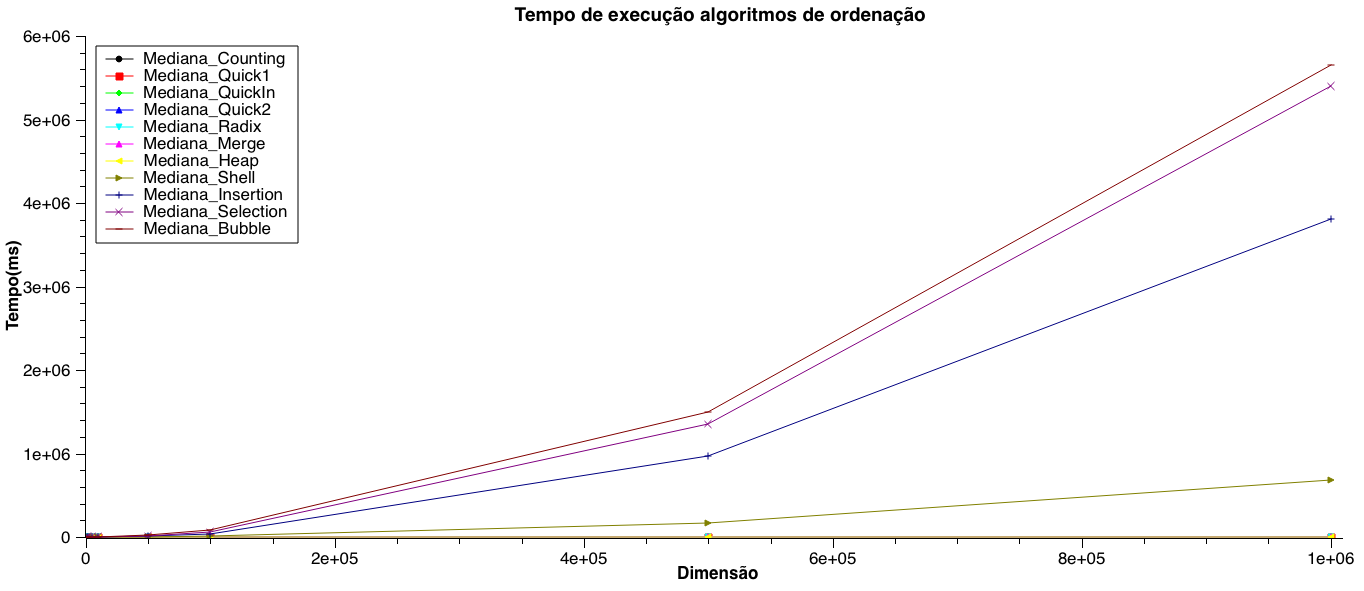
\includegraphics[scale=0.25]{algoritmos.png}
	\caption{Gráfico das medianas de cada algoritmo em função da dimensão}
	\label{Rotulo}
\end{figure}
\begin{figure}
	\centering
	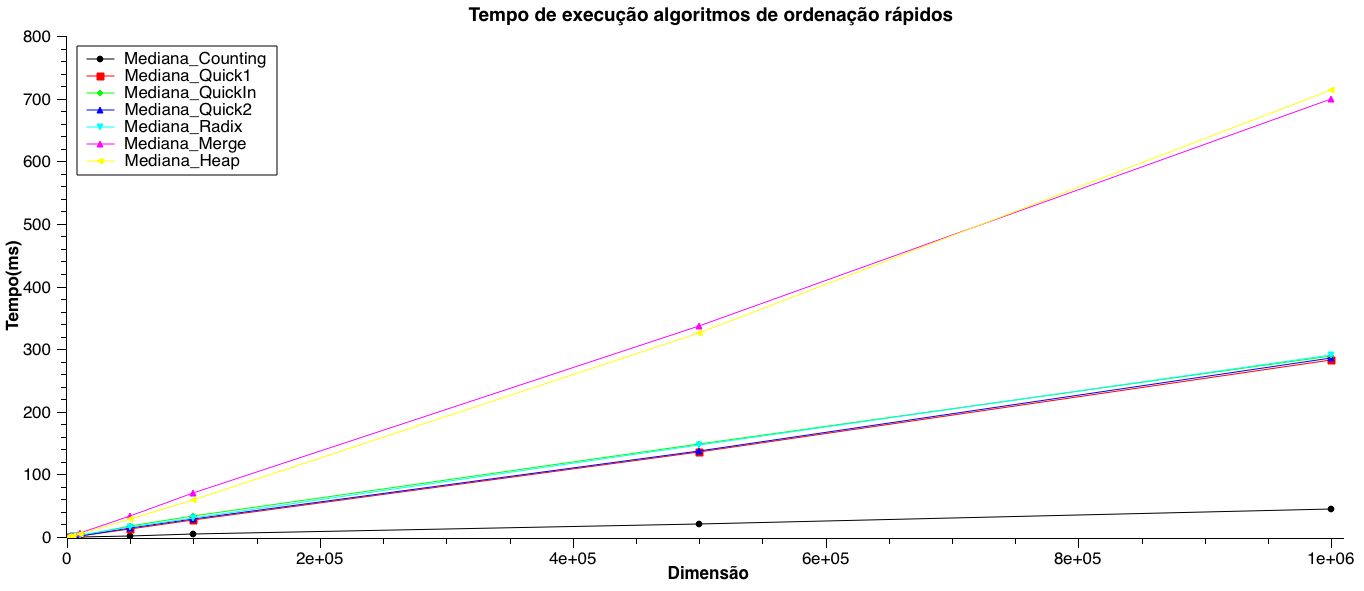
\includegraphics[scale=0.25]{algoritmosrapidos.png}
	\caption{Gráfico das medianas de cada algoritmo rápido em função da dimensão}
	\label{Rotulo}
\end{figure}
\begin{figure}
	\centering
	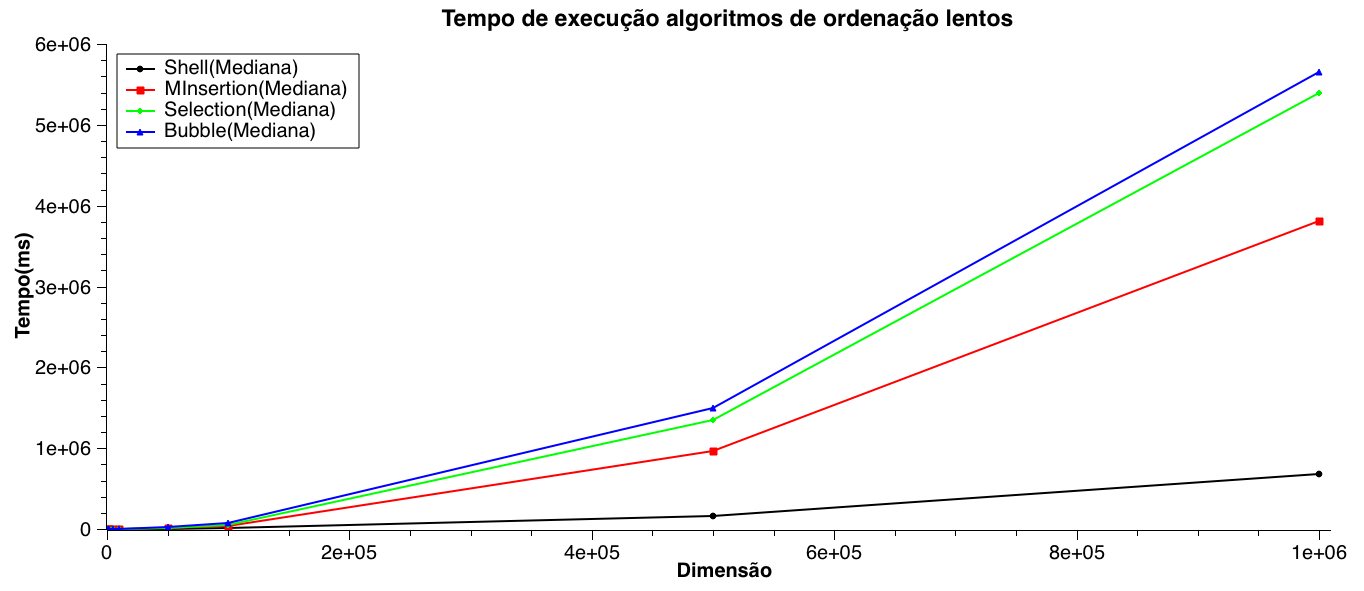
\includegraphics[scale=0.25]{algoritmoslentos.png}
	\caption{Gráfico das medianas de cada algoritmo lento em função da dimensão}
	\label{Rotulo}
\end{figure}
\clearpage
\section{Considerações Finais}
Os resultados atingidos foram satisfatórios e foram os resultados esperados visto a ordem de complexidade de cada algoritmo, entretanto o \textit{Counting Sort} foi uma surpresa, pois seu resultado superou o quick sort, isso é devido a sua facilidade para ordenar inteiros que se conhece o intervalo e ajuda o fato dele nao percorrer o vetor procurando o minimo e o máximo.
\end{document}